\chapter{OpenStack Folsom}\label{cap:openstack}
\noindent The current section intends to detail the IaaS Cloud implementation that has been chosen: OpenStack. Initially, a global vision will be given to the reader, to progressively focus on its constituent modules' responsibilities and how they collaborate to maintain the service running.

\section{Global Architecture}\label{sec:arquitecturaglobal}
\noindent Figure \ref{fig:arquitecturaos} shows the three basic operational components of OpenStack Folsom:

\begin{description}
 \item[Functional Core:] OpenStack Compute, OpenStack Quantum and OpenStack Storage (Cinder and Swift).
 \item[Web Management Interface:] OpenStack Horizon.
 \item[Shared Services:] OpenStack Glance, OpenStack Keystone and other related services like a DBMS for persisting meta-data or a messaging queue.
\end{description}

\begin{figure}[tbp]
\begin{center}
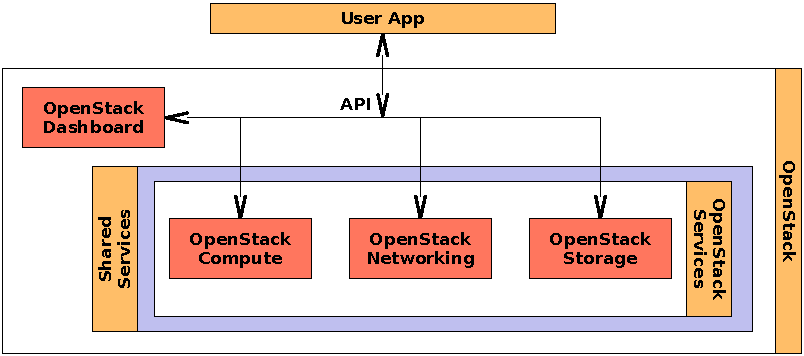
\includegraphics[width=0.9\textwidth]{imagenes/012.pdf}
 \caption{OpenStack Arquitecture}
\label{fig:arquitecturaos}
\end{center}
\end{figure}

The different components have been devised to run in a shared nothing fashion. This provides the cloud admin the flexibility required to distribute the modules over the cluster as pleased. An example of a particular OpenStack deployment is shown in figure \ref{fig:despliegueos}. What it is missing from the diagram, for clarity, is the asynchronous queue that mediates inter-module communication. Qpid and RabbitMQ are the two queue implementations that are officially documented, being the former the one that we used in our test deployment.

\begin{figure}[tbp]
\begin{center}
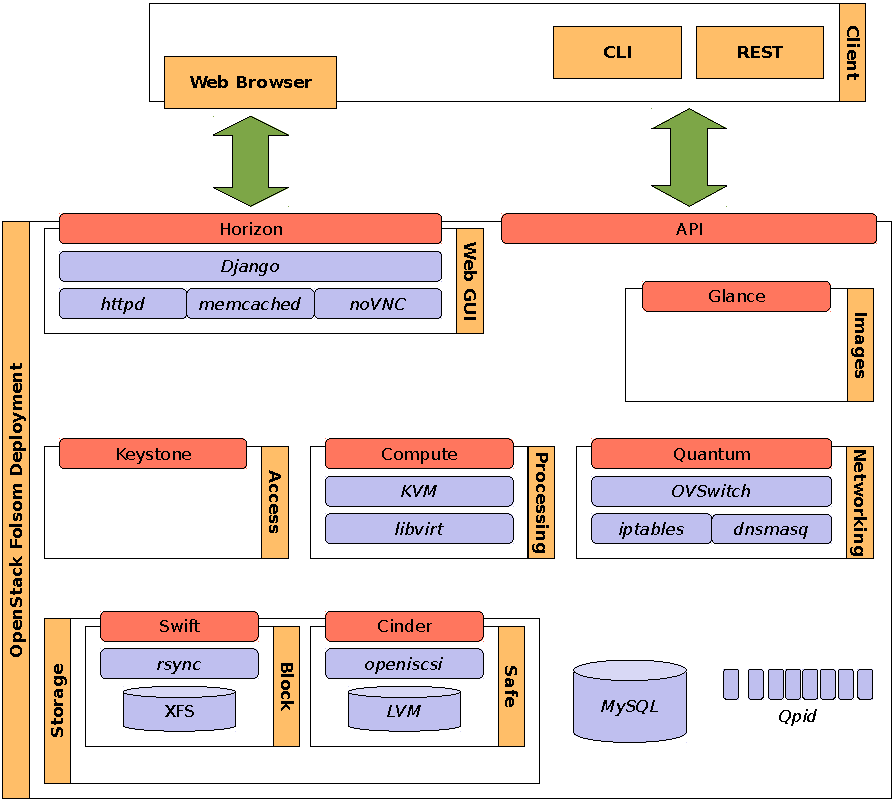
\includegraphics[width=0.99\textwidth]{imagenes/011.pdf}
 \caption{Example of an OpenStack Folsom deployment}
\label{fig:despliegueos}
\end{center}
\end{figure}

\section{Horizon}\label{sec:horizon}
\noindent Horizon represents the fundamental window to set up the cloud. As discussed in the previous section, Horizon does not currently --- as of Folsom version --- present a global view of the physical infrastructure, leaving the user in the dark in this respect. Horizon is written in Python on top of \texttt{Django}, the web framework. Django itself relays on a web server like \texttt{httpd} to expose static files, uses a caching mechanism (\texttt{memcached}) to speedup load times and a terminal embedding (\texttt{noVNC}) system to view the output of the virtual graphic card directly on Horizon.

To manage and create instances in the cloud, OpenStack gives the cloud admin the ability to register authorization roles that will let the users consume those services whose role give access to. While the admin is allowed to sign up custom roles, two roles that ship the distribution are the \emph{Cloud Admin} and the \emph{Cloud Member}.

A user granted the admin role will be able to manage:

\begin{description}
 \item[Tenants:] Create, delete, member users, alter quotas, etc.
 \item[Users:] Create, modify or delete.
 \item[OS Images:] List, remove or modify meta-data.
 \item[Instances:] Reset, shutdown, suspend, print log on screen, etc.
 \item[Volumes:] Create, list, attach to an instance, etc.
 \item[Networks:] Create, modify or delete.
\end{description}

A user granted the member role will be able to:

\begin{description}
 \item[Status:] Quota, resources, etc.
 \item[Instances:] create, shutdown, reset, suspend, print log, create image from a running instance (snapshot), etc.
 \item[Volumes:] List, create, modify, attach to an instance, create a volume snapshot, etc.
 \item[Images:] Create, list, delete, modify, etc.
 \item[Networking:] Manage public IPs (floating IPs).
 \item[Security groups:] Create, delete or modify security rules.
 \item[Keypairs:] Create, modify or delete.
\end{description}

\section{Keystone}\label{sec:keystone}

\noindent Keystone is the central security check point and information repository storing information needed to access the cloud installed services. It verifies, before each request, user credentials and authorizations in OpenStack services. Keystone divides this functionality in two parts: on the one hand user control, on the other service catalog.

To deal with users, Keystone assigns them tenants or projects. Users, as discussed above, are granted the membership to a tenant and a service quota they will have to adhere to; they are also restricted to the tenant quota.

To organize the catalog at hand Keystone defines two other concepts within the service catalog: \emph{Services} and \emph{endpoints}. A service in the catalog is a mere abstract description of an exploitable cloud feature by the user. The particular implementation of the service is managed by the set of endpoints associated to it. Said collection contains every piece of information that is required for users to consume the services. Figure \ref{fig:secuenciais} shows a Sequence Diagram portraying the interchanged messages between the different entities taking part to consume a service: \emph{Create a new instance}.

\begin{figure}[tbp]
\begin{center}
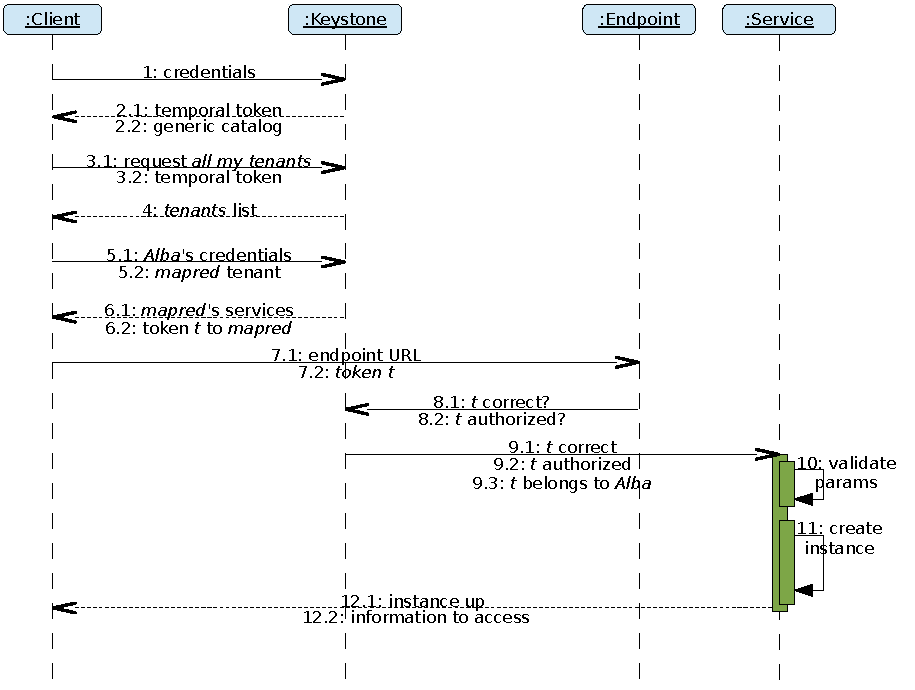
\includegraphics[width=0.99\textwidth]{imagenes/013.pdf}
 \caption{Sequence Diagram --- create instance}
\label{fig:secuenciais}
\end{center}
\end{figure}

Stemming from the fact the Horizon exposes only a part of OpenStack functionality, to help dealing with security Keystone installs a CLI tool to interact with the REST service in charge of administrative operations. Issuing certain commands to Keystone through a terminal requires the knowledge of the admin token, which has to be conveniently secured, or the login credentials of a user with the admin role. Lastly, it should be noted that Keystone uses a data base to store user access credentials and the service catalog meta-data.

\section{Quantum}\label{sec:quantum}

\noindent Starting with Folsom, Quantum is the module to manage virtual networking. It was introduced to separate the networking part from the computing part, held together in \texttt{Compute} module. Certainly, the fact that it had been refactored out demonstrates OpenStack's evolving model toward a more coherent less coupled functional allocation; and as it is independent, it could be configured in a dedicated node.

To bring virtual networking into existence Quantum banks on external plug-ins. Two of those plug-ins whose usage is covered in the official Quantum administrator manual (\cite{quantumadminfolsom}) are \texttt{OpenVSwitch} and \texttt{LinuxBridge}. Additionally, Quantum relies on iptables to configure routing rules and firewall, \texttt{dnsmasq} for the \emph{DNS}, the \emph{DHCP} and the \emph{NAT}.

Figure \ref{fig:desplieguequantum} pictures a topology example of a virtual network. On it, \emph{30.0.0.X} represent public IPs and \emph{10.0.X.Y} private. This virtual network assigns a virtual router to each tenant but more could be added with ease. Private IP overlapping over different networks is possible as expected (\emph{10.0.0.2}). The routers public IPs --- they could be assigned more external interfaces --- must be taken from the external network (\emph{30.0.0.0}).

\begin{figure}[tbh]
\begin{center}
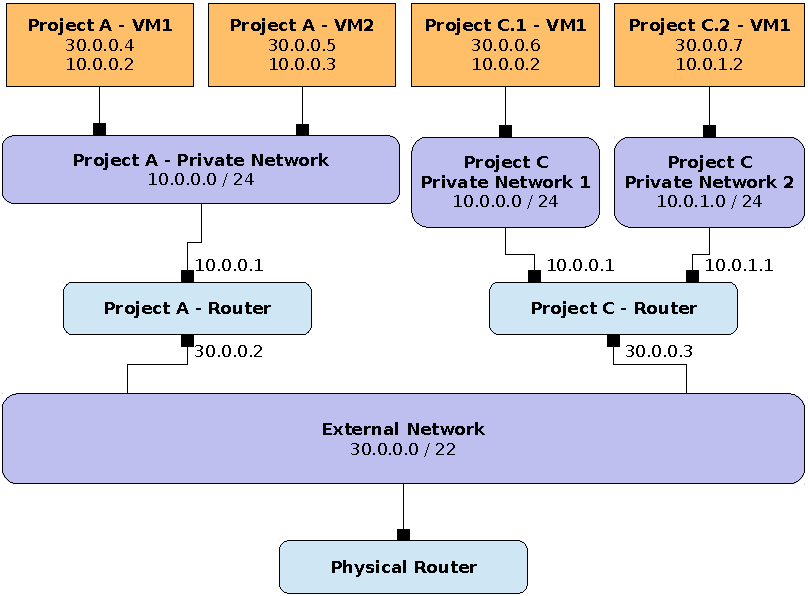
\includegraphics[width=0.9\textwidth]{imagenes/014.pdf}
 \caption{Virtual network deployment with Quantum}
\label{fig:desplieguequantum}
\end{center}
\end{figure}

\section{Compute}\label{sec:compute}

\noindent Compute is the central module. Its duty entails orchestrating the global workings in the cloud, delegating each particular function to the service on charge. In the end, Compute will let a logged user start virtual instances, which will draw their VCPU, VRAM and VHDD from the physical cluster. Yet required, Compute does not contain a virtualization package. The approach is to delegate infrastructure provision to a hypervisor found typically, but not restricted to, in the same node. To expose this on-demand computational service, Compute implements a REST API so that users can control their instances' life cycle directly from a REST client (like the CLI tools that accompany Compute).

To create an instance in effect, Compute will communicate with other modules within the cloud to orchestrate the execution and, finally, it will pass the request to the most suitable cluster node's hypervisor --- most suitable according to the cloud-defined rule set --- that will bring up the VM. Some of the supporting services are described below.

\begin{description}
 \item[Keystone:] Collates credentials y authorizes requests.
 \item[Glance:] Selects the OS image that will be used to start the VM.
 \item[Quantum:] Grants private and public IPs as well as manages instance network traffic.
 \item[Cinder:] Manages block storage and on-line volume attachments.
 \item[Qpid:] Handles message interchange between Keystone, Quantum, Glance and/or Cinder.
\end{description}

As it has been discussed all along, if there is some trait that aligns different IaaS Cloud implementations is their flexibility. Users' computational needs are as diverse as they are changing and therefore they expect to be given the chance to define virtual infrastructure adapting to those needs. In OpenStack, each possible particular configuration instance will take its VCPU, RAM and VHDD from a cluster host, and the users will be allowed to shape those to their requirements with ease.

\section{Glance}\label{sec:glance}
\noindent Glance is OpenStack's OS image storage service. Glance may be configured to drive images stored in a myriad of backends, ranging from Swift to an HTTP-addressable location. As happens with every other OpenStack module, Glance relies on Keystone to grant access to the images, and coordinates its operation with Compute to put them in execution on demand.

Glance supports a good number of image and container types --- this fact being merely informative to the Cloud framework as it is the hypervisor who would have to support the particular combination image type, container type ---, and they are stored as metadata linked to the image in Glance.

\section{Storage}\label{sec:almacenamiento}
\noindent OpenStack provides three main options regarding storage types:

\begin{description}
 \item[Ephemeral:] The size of the drive hosting the root file system is set following the particular flavor parameters when the VM starts. The files contained in this file system are those present in the image file stored in Glance. Any alteration to this file system will only persist the execution of the VM. Any change on the image files is written temporarily to be discarded as soon as the VM is shut down.
 \item[Block:] By making use of storage volumes managed by Cinder with \emph{LVM} (\emph{Logical Volume Manager}) OpenStack provides the ability to attach indeterminably-sized logical volumes to instances on-demand. This store kind guaranties that information is preserved between VM executions. However, this method carries an important handicap, that of being unable to attach a single volume to two different instances at the time. High availability or data safety on failure are not supported, as data is stored in a single place. A backup or RAID policies may be established to get over these limitations but they are discouraged as OpenStack has it own module to deal with them.
 \item[Safe:] Swift manages a safe distributed storage banking on controlled replication allowing for high availability deployments that overcome hard drive's inherent fragility. Swift draws on \texttt{rsync} to synchronize \emph{XFS} partitions.
\end{description}

\subsection{Cinder}\label{subsec:cinder}
\noindent Cinder is the OpenStack module that takes care of virtual block storage devices --- functionally similar to Amazon's \emph{EBS} (\emph{Elastic Block Storage}). Cinder uses an \emph{iSCSI} implementation (\texttt{open-iscsi}) and LVM to manage operations on the volumes. Creation, attachment and detachment, and logical volume removal is directly controlled through Horizon.

Those persistent virtual blocks are administered as logical volumes pertaining to a volume group controlled by Cinder. Cinder, though, shall not be used to create a shared medium to instances, as \emph{NFS} (\emph{Network File System}) or a \emph{SAN} (\emph{Storage Area Network}) solution do; for a single volume cannot be attached to different instances at the same time. An interesting option that Cinder opens is using a logical volume to boot instances, therefore sharing the set of files contained in the image among them.

\subsection{Swift}\label{subsec:swift}
\noindent Just as happened with Cinder, Swift cannot be framed into traditional shared networking nor  be compared to Cinder: Swift covers a different functional demand. Swift is defined as ``\texttt{a scalable object storage system where logged users control their store buckets uploading, downloading or deleting files to their will}'' \cite{osswift}. Swift may be conceived as a functional clone to Amazon's S3 or Eucaliptus' \texttt{Walrus}, implementing a partially Amazon-compatible REST API. Central to Swift's implementation is replication.

\subsubsection{Replication}\label{subsubsec:replicacion}
\noindent Scalability, fault tolerance, high availability, safety, storage and load balancing are some distinguishing features of Swift's. As discussed, high availability and fault tolerance are implemented with replication. Replication is a mechanism by which a distributed system keeps block copies at different locations of the deployment to guarantee better performance and limit failure impact.

Within Swift, replication processes on every \emph{Object Server} --- any node in the cluster configured to support them --- periodically compare their local blocks with remote replicas to collate their update state. Comparing replicas states is as costly a process as it is often, thus \emph{Hash lists} and \emph{watermark}s are used to improve comparison time. Replication is transparent to the user and Rsync or HTTP transport replica payload across the cluster. When a new Swift node is added to the cluster, replica distribution becomes unbalanced and will trigger automatic rebalancing. When it be synchronized with the cluster, the new node will be able to respond to data requests.

\subsubsection{Updaters y Auditors}\label{subsubsec:otroscompswift}
\noindent Other supporting services that complete the functional circle defined for Swift are \emph{Updater}s and \emph{Auditor}s. The former act when a replica synchronization error is raised or when Object Servers load is so high to make a data request stay unreplied. It happens then that the execution of this operation is delayed and queued, being serviced by the Updater process at a later time. Auditors continually scan the file system looking for integrity failures in objects or buckets. If an inconsistency were to be found, the incoherent entity would quarantined and replicas would be made anew.
